
\RequirePackage{amsmath}
\DeclareMathOperator*{\argmax}{arg\,max}
\DeclareMathOperator*{\argmin}{arg\,min}
\documentclass{svjour3}
\usepackage{float}
\usepackage[margin=1in]{geometry}
\usepackage[numbers, sort&compress]{natbib}
\usepackage{pdfpages}
\usepackage{rotating}
\usepackage{relsize}
\usepackage{graphicx}
\usepackage{booktabs}
\usepackage[strings]{underscore}
\usepackage{anyfontsize}
\usepackage{subfigure}
\usepackage{lipsum}
\usepackage[utf8]{inputenc}

\begin{document}

\abstract


\section{Introduction}
  
  
\section{Methodology}
The goal of the models presented in this paper is to predict the number of fires that occur in each census tract in the dataset over a five-year ``test" interval, comprising of the years 2012-2016 (inclusive). All models are strictly informed only by records that were completed prior to the end of the year 2011. This includes geocoded NFIRS data for residential fires that occurred the training interval, as well as the population, demographic, and housing unit information reported in the 2006-2010 American Community Survey 5-year estimates. Training the models using only data completed prior to the testing interval allows for the evaluation of the models' ability to make future predictions.


\section{Modeling overview}
The theoretical framework common to all models is that the occurrence of residential fires within each department follows a spatially inhomogeneous point process with an intensity function $\lambda_{i}(\textbf{x})$ 
where \textbf{x} is a point located in $\textbf{R}^2$ within the coverage area of department \textit{i}. $\Lambda_{i,j}$, described in equation \ref{eqn:rate_description}:

\begin{equation}
  \label{eqn:rate_description}
  \Lambda_{i,j} = \int_{B_{i,j}} \lambda_{i}(\textbf{x})d\textbf{x}
\end{equation}

\noindent where $B_{i,j}$ is the geographic area of census tract \textit{i,j}. Each of the models provides the estimated average rate of residential fires at the census tract level, $\hat\Lambda_{ij}$. Because this quantity is assumed to be temporally homogeneous\footnote{Note that in the most general sense, the intensity can also vary temporally such that $\lambda_i = \lambda_i(\textbf{x},t)$. Although the authors made various attempts to estimate the temporal evolution of $\lambda_i$, the large variance in the count data made it difficult to infer transient trends from the 6-year training interval that improve predictions relative to the assumption that $\lambda_i$ is temporally homogeneous.}, the prediction for the number of fires that occur during the test interval is then calculated according to equation \ref{eqn:rate_integral}: 

\begin{equation}
  \label{eqn:rate_integral}
  \hat{f}_{test,i,j} = \int_{0}^{n_{test}}\hat\Lambda_{i,j}dt
  = n_{test}\hat\Lambda_{i,j}
\end{equation}

\noindent where $n_{test}$ is the duration of the test interval (5 years) and $\hat{f}_{test,i,j}$ is the predicted number of fires that occur during the test interval.

Then the efficacy of a model's prediction is then quantified using the Poisson deviance, which is calculated according to equation \ref{eqn:deviance}:

\begin{equation}
  \label{eqn:deviance}
  D_i = 2\sum_{j=1}^{N_i}\bigg[
   f_{test,i,j}log\big(\frac{f_{test,i,j}}{\hat{f}_{test,i,j}}\big) - 
   (f_{test,i,j}-\hat{f}_{test,i,j}) 
  \bigg]
\end{equation}

\noindent where $N_i$ is the number of census tracts covered by department \textit{i}, $f_{test,i,j}$ is the number of residential fires that actually occurred in census tract \textit{i,j} during the 5-year test interval A lower deviance indicates more accurate predictions, with a deviance of zero corresponding to a model that perfectly predicted the number of residential fires that occurred in each census tract during the test interval.



\subsection{Spatial models}
The section outlines two purely spatial models that utilize only the locations of past fire in order to forecast future fire counts at the census tract level. The first is a naive ``spatial histogram'' model that serves as a performance baseline for all subsequent models described in this paper. The second employs Kernel Density Estimation (KDE), which is a statistical method commonly used to generate incident heatmaps. 

\subsubsection{Naive count forecasting (spatial histogram)}
The simplest forecasting technique described in this paper is a naive count model that can be thought of as a spatial histogram with the census tracts representing a set of non-uniform bins. The estimate for the count density rate in census tract \textit{j} covered by fire department \textit{i} is described by equation \ref{eqn:naive_count}:

\begin{equation}
  \label{eqn:naive_count}
  \hat{\Lambda}_{count,i,j} = \frac{f_{train,i,j}}{n_{train}} 
\end{equation}

\noindent where $\hat{\Lambda}_{count,i,j}$ is the estimated average fire density per year, $f_{train,i,j}$ is the total number of fires in census tract \textit{i, j} that occurred during the training interval, $n_{train}$ is the number of years that comprise the training interval (6 years), and $A_{i,j}$ is the land area of census tract \textit{i, j}. As an example, if 12 residential fires occurred in a census tract during the 6-year training interval (2 fires/year), then this framework would predict that 10 fires would occur in that census tract during the subsequent 5-year test interval. This methodology serves as a performance baseline for the more sophisticated forecasting models described later in this paper. An illustration of this methodology is provided in Figure \ref{fig:spatial_histogram}. 


\begin{figure}[htb] \centering
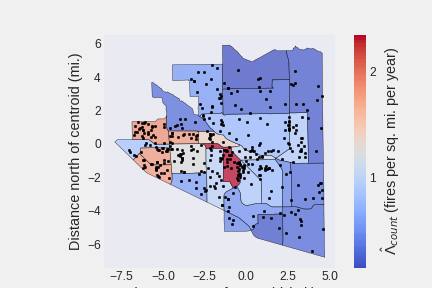
\includegraphics[width=.5\textwidth]{./figures/spatial_histogram.png}
\caption{A visual depiction of the naive count forecasting methodology for an example department. The black dot markers indicate the location of a residential fire that occurred during the six-year training interval, 2006-2011 (inclusive). The color corresponds to the fire count density rate estimated from this approach. Notice that large census tracts with few fires have the lowest density rate and small tracts with many fires have the highest density rate.}
\label{fig:spatial_histogram}
\end{figure}

\subsubsection{Kernel density estimation}
The second spatial model discussed in this paper is Kernel density estimation (KDE), which is a statistical methodology for inferring a density distribution from a set of point observations. This is the framework commonly used to generate incident heatmaps. The major difference between this method and the one outlined in the previous section is that KDE results  a smoothed surface that does not arise from ``binning" the incidents into discrete areas such as the census tract boundaries. Instead, this density surface is generated by centering a kernel function on each point (i.e. residential fire location) in the training set. The density function can then be calculated at any location by summing the kernel functions of all past residential fires at that location. This process is described by equation \ref{eqn:kde}:

\begin{equation}
  \label{eqn:kde}
  \hat\lambda_{i,KDE}(\textbf{x}) = \frac{1}{n_{train}}\sum_{m=1}^{F_i}K_i(\textbf{x},\tilde{\textbf{x}}_{i,m})
\end{equation}

\noindent where $F_i$ is the total number of fires that occurred during the training interval, and $\tilde{\textbf{x}}_{i,m}$ is the location of the $m^{th}$ residential fire that occured during the training interval in the coverage area of department \textit{i}. Note that the subscript \textit{j} is not used here because $\hat\lambda_{i,KDE}(\textbf{x})$ does not depend on census tract geometries. $K_i(\textbf{x},\tilde{\textbf{x}}_{i,m})$ is a department-specific kernel function. The KDE predictions described in this paper were obtained using a two-dimensional isotropic Gaussian kernel, described in equation \ref{eqn:gaussian_kernel}:


\begin{equation}
  \label{eqn:gaussian_kernel}
  K_i(\textbf{x},\tilde{\textbf{x}}_{i,m}) = \frac{1}{2\pi b_{i}^2}exp\bigg(\frac{d^2_i(\textbf{x},\tilde{\textbf{x}}_{i,m})}{2b_{i}^2}\bigg)
\end{equation}

\noindent where $d_i(\textbf{x},\tilde{\textbf{x}}_{i,m})= ||\textbf{x} - \tilde{\textbf{x}}_{i,m}||_2$, the euclidean distance between an arbitrary point \textbf{x} and $\tilde{\textbf{x}}_{i,m}$. $b_i$ is the department-specific bandwidth. Loosely speaking, it represents the length scale over which past fires elevate the estimated fire risk of surrounding areas. An important attribute of the kernel used in these analyses is that $\int_{\textbf{x} \in \textbf{R}^2}K_i(\textbf{x},\tilde{\textbf{x}}_{i,m})d\textbf{x} = 1$, and by extension, $n_{train}\int_{\textbf{x} \in \textbf{R}^2}\hat\lambda_{i,KDE}(\textbf{x}) d\textbf{x} = F_i$. In other words, the total kernel density is equal to the total number of fires that occurred during the training interval. In order to provide intuition for the reader, a simplified illustration of the KDE approach is provided in Figure \ref{fig:1dkde}.

\begin{figure}[htb] \centering
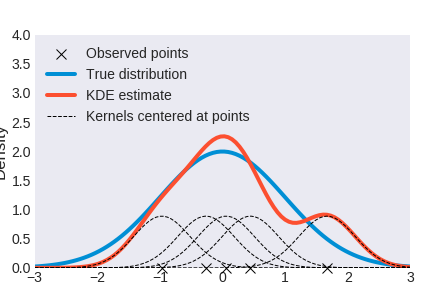
\includegraphics[width=.5\textwidth]{./figures/1dkde.png}
\caption{A simplified one-dimensional illustration of the KDE method. Although the locations of residential fires are defined in $\textbf{R}^2$, the use of a location coordinate defined in $\textbf{R}$ allows for an intuitive visualization. Five points (indicated by the ``X" markers) are drawn from a standard normal distribution, so that the true density function (the blue curve) is five times the standard normal probability distribution. The dashed black curves indicate Gaussian kernels centered on each point, and the red curve shows the KDE result, which is the sum of the kernels.}
\label{fig:1dkde}
\end{figure}

A key consideration for generating meaningful results from KDE is the selection of the bandwidth parameter, $b_i$. Selecting too small of a bandwidth results in density estimates that have highly localized peaks that correspond to the locations of past incidents; conversely, selecting too large of a bandwidth results in an overly smoothed density estimate that tends towards a uniform density profile as $b_i \rightarrow  \infty$. Figure \ref{fig:band_comparison} shows the effect of different bandwidth on the resulting KDE heatmaps along with the "optimized bandwidth" which is obtained through 5-fold cross validation. This technique randomly splits the training data into five groups of approximately equal size. Using a specific value for $b_i$, a KDE map is generated using the data from four of the five groups or folds. The algorithm then determines the likelihood of the the locations of the fires in the excluded fold using the map generated from incidents in the four remaining folds. This likelihood arises from the fact that $\frac{n_{train}}{F_i}\hat\lambda_{i,KDE}(\textbf{x})$ is actually an estimate of the probability density function for the location of a new fire. This process is then repeated so that each of the five folds are excluded, and 100 logarithmically spaced values of $b_i$ are evaluated over the interval $[0.01,10]$ miles and the bandwidth that generated KDE maps with the highest predictive accuracy is chosen as the optimal bandwidth, $b_{i,opt}$. This optimization process is described mathematically by equation \ref{eqn:fivefold}:

\begin{equation}
  \label{eqn:fivefold}
   b_{opt,i} = \argmax_{b_i} \prod_{k=1}^5 \prod_{m \in E_k}   \hat\lambda_{i,k}(\tilde{\textbf{x}}_m,b_i)
\end{equation}


\noindent where $\hat\lambda_{i,k}(\tilde{\textbf{x}}_m,b_i)$ is the KDE function that is generated using a bandwidth of $b_i$ and also excluding incidents in the k$^{th}$ fold, $E_k$. 

\begin{figure}[!htb]
       \begin{center}
  %
          \subfigure[$b_i=0.1$ mi]{%
              \label{fig:smallband} 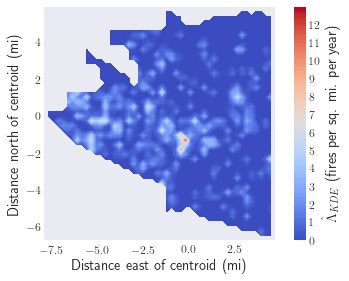
\includegraphics[width=5cm,keepaspectratio]{figures/small_band.png}
          }%
          \subfigure[$b_i= 1.0$ mi]{%
             \label{fig:largeband} 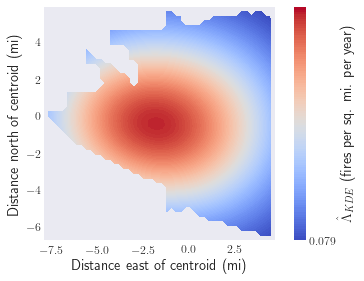
\includegraphics[width=5cm,keepaspectratio]{figures/large_band.png}
          } % 
            \subfigure[$b_i=b_{i,opt}=0.43$ mi]{%
             \label{fig:optband} 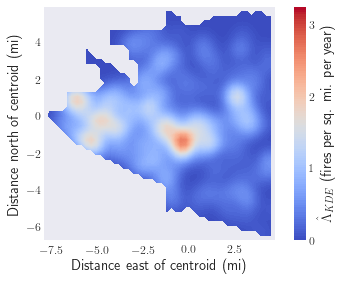
\includegraphics[width=5cm,keepaspectratio]{figures/correct_band.png}
          } % ------- End of the first row ----------------------%
      \end{center}
      \caption{ Visual depiction of the effect of different bandwidth values for heatmaps generated from KDE. The bandwidth is too small in \protect\subref{fig:smallband}, which is apparent from the many localized ``hotspots."  Conversely, the bandwidth is too large in \protect\subref{fig:largeband}, and the result is an overly smoothed heatmap. \protect\subref{fig:optband} shows the heatmap with the optimized bandwidth.}
     \label{fig:band_comparison}
  \end{figure}

The results from the optimizations give insight into the distances over which fire risk factors vary with the departments in the dataset. 

\begin{figure}[!htb]
       \begin{center}
  %
          \subfigure[$b_i=0.1$ mi]{%
              \label{fig:bhist} 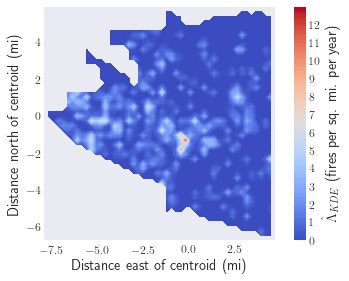
\includegraphics[width=5cm,keepaspectratio]{figures/small_band.png}
          }%
          \subfigure[$b_i= 1.0$ mi]{%
             \label{fig:largeband} 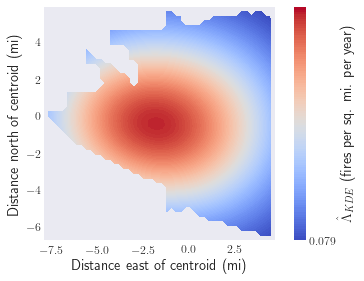
\includegraphics[width=5cm,keepaspectratio]{figures/large_band.png}
          } % 
           % ------- End of the first row ----------------------%
      \end{center}
      \caption{ Visual depiction of the effect of different bandwidth values for heatmaps generated from KDE. The bandwidth is too small in \protect\subref{fig:smallband}, which is apparent from the many localized ``hotspots."  Conversely, the bandwidth is too large in \protect\subref{fig:largeband}, and the result is an overly smoothed heatmap. \protect\subref{fig:optband} shows the heatmap with the optimized bandwidth.}
     \label{fig:band_comparison}
  \end{figure}
















\clearpage
\bibliographystyle{unsrtnat}
\bibliography{./papers/references}
\end{document}
